\documentclass[journal,12pt,twocolumn]{IEEEtran}

\usepackage{setspace}
\usepackage{gensymb}
\singlespacing
\usepackage[cmex10]{amsmath}
\usepackage{amssymb}
\usepackage{xurl}
\usepackage{tabularx}
\usepackage{amsthm}
\usepackage{comment}
\usepackage{mathrsfs}
\usepackage{txfonts}
\usepackage{stfloats}
\usepackage{bm}
\usepackage{cite}
\usepackage{cases}
\usepackage{subfig}

\usepackage{longtable}
\usepackage{multirow}

\usepackage{enumitem}
\usepackage{mathtools}
\usepackage{steinmetz}
\usepackage{tikz}
\usepackage{circuitikz}
\usepackage{verbatim}
\usepackage{tfrupee}
\usepackage[breaklinks=true]{hyperref}
\usepackage{graphicx}
\usepackage{tkz-euclide}

\usetikzlibrary{calc,math}
\usepackage{listings}
    \usepackage{color}                                            %%
    \usepackage{array}                                            %%
    \usepackage{longtable}                                        %%
    \usepackage{calc}                                             %%
    \usepackage{multirow}                                         %%
    \usepackage{hhline}                                           %%
    \usepackage{ifthen}                                           %%
    \usepackage{lscape}     
\usepackage{multicol}
\usepackage{chngcntr}

\DeclareMathOperator*{\Res}{Res}

\renewcommand\thesection{\arabic{section}}
\renewcommand\thesubsection{\thesection.\arabic{subsection}}
\renewcommand\thesubsubsection{\thesubsection.\arabic{subsubsection}}

\renewcommand\thesectiondis{\arabic{section}}
\renewcommand\thesubsectiondis{\thesectiondis.\arabic{subsection}}
\renewcommand\thesubsubsectiondis{\thesubsectiondis.\arabic{subsubsection}}


\hyphenation{op-tical net-works semi-conduc-tor}
\def\inputGnumericTable{}                                 %%

\lstset{
%language=C,
frame=single, 
breaklines=true,
columns=fullflexible
}
\begin{document}


\newtheorem{theorem}{Theorem}[section]
\newtheorem{problem}{Problem}
\newtheorem{proposition}{Proposition}[section]
\newtheorem{lemma}{Lemma}[section]
\newtheorem{corollary}[theorem]{Corollary}
\newtheorem{example}{Example}[section]
\newtheorem{definition}[problem]{Definition}

\newcommand{\BEQA}{\begin{eqnarray}}
\newcommand{\EEQA}{\end{eqnarray}}
\newcommand{\define}{\stackrel{\triangle}{=}}
\bibliographystyle{IEEEtran}
\raggedbottom
\setlength{\parindent}{0pt}
\providecommand{\mbf}{\mathbf}
\providecommand{\pr}[1]{\ensuremath{\Pr\left(#1\right)}}
\providecommand{\qfunc}[1]{\ensuremath{Q\left(#1\right)}}
\providecommand{\sbrak}[1]{\ensuremath{{}\left[#1\right]}}
\providecommand{\lsbrak}[1]{\ensuremath{{}\left[#1\right.}}
\providecommand{\rsbrak}[1]{\ensuremath{{}\left.#1\right]}}
\providecommand{\brak}[1]{\ensuremath{\left(#1\right)}}
\providecommand{\lbrak}[1]{\ensuremath{\left(#1\right.}}
\providecommand{\rbrak}[1]{\ensuremath{\left.#1\right)}}
\providecommand{\cbrak}[1]{\ensuremath{\left\{#1\right\}}}
\providecommand{\lcbrak}[1]{\ensuremath{\left\{#1\right.}}
\providecommand{\rcbrak}[1]{\ensuremath{\left.#1\right\}}}
\theoremstyle{remark}
\newtheorem{rem}{Remark}
\newcommand{\sgn}{\mathop{\mathrm{sgn}}}
\providecommand{\abs}[1]{\vert#1\vert}
\providecommand{\res}[1]{\Res\displaylimits_{#1}} 
\providecommand{\norm}[1]{\lVert#1\rVert}
%\providecommand{\norm}[1]{\lVert#1\rVert}
\providecommand{\mtx}[1]{\mathbf{#1}}
\providecommand{\mean}[1]{E[ #1 ]}
\providecommand{\fourier}{\overset{\mathcal{F}}{ \rightleftharpoons}}
%\providecommand{\hilbert}{\overset{\mathcal{H}}{ \rightleftharpoons}}
\providecommand{\system}{\overset{\mathcal{H}}{ \longleftrightarrow}}
	%\newcommand{\solution}[2]{\textbf{Solution:}{#1}}
\newcommand{\solution}{\noindent \textbf{Solution: }}
\newcommand{\cosec}{\,\text{cosec}\,}
\providecommand{\dec}[2]{\ensuremath{\overset{#1}{\underset{#2}{\gtrless}}}}
\newcommand{\myvec}[1]{\ensuremath{\begin{pmatrix}#1\end{pmatrix}}}
\newcommand{\mydet}[1]{\ensuremath{\begin{vmatrix}#1\end{vmatrix}}}
\newcommand*{\permcomb}[4][0mu]{{{}^{#3}\mkern#1#2_{#4}}}
\newcommand*{\perm}[1][-3mu]{\permcomb[#1]{P}}
\newcommand*{\comb}[1][-1mu]{\permcomb[#1]{C}}
\numberwithin{equation}{subsection}
\makeatletter
\@addtoreset{figure}{problem}
\makeatother
\let\StandardTheFigure\thefigure
\let\vec\mathbf
\renewcommand{\thefigure}{\theproblem}
\def\putbox#1#2#3{\makebox[0in][l]{\makebox[#1][l]{}\raisebox{\baselineskip}[0in][0in]{\raisebox{#2}[0in][0in]{#3}}}}
     \def\rightbox#1{\makebox[0in][r]{#1}}
     \def\centbox#1{\makebox[0in]{#1}}
     \def\topbox#1{\raisebox{-\baselineskip}[0in][0in]{#1}}
     \def\midbox#1{\raisebox{-0.5\baselineskip}[0in][0in]{#1}}
\vspace{3cm}
\title{AI1103 : Assignment 5}
\author{Raja Ravi Kiran Reddy - CS20BTECH11009}
\maketitle
\newpage
\bigskip
\renewcommand{\thefigure}{\arabic{figure}}
\renewcommand{\thetable}{\arabic{table}}
Download all python codes from 
\begin{lstlisting}
https://github.com/BokkaRajaRaviKiranReddy/AI1103/tree/main/Assignment5/codes
\end{lstlisting}
%
and latex codes from 
%
\begin{lstlisting}
https://github.com/BokkaRajaRaviKiranReddy/AI1103/blob/main/Assignment5/Assignment5.tex
\end{lstlisting}
\section*{GATE 2021 ME-set1-Q18}
Activities A,B,C,D from the critical path for a project with a PERT network. The means an variances of the activity duration for each activity are given below . All activity duration follow the Gaussian (normal) distribution,and are independent of each other.

\begin{table}[h!]
\centering
\begin{tabular}{|c||c|c|c|c|}
    \hline
    Activity & A& B& C& D \\
    \hline
    %& & &\\
    Mean & 6& 11& 8& 15\\[1ex]
    \hline
    %& & &\\
    variance & 4& 9& 4& 9\\[1ex]
    \hline
\end{tabular}
\end{table}
The probability that the project will be completed within 40 days is  

(round off to two decimal places)

(Note: Probability is a number between 0 and 1)
\section*{SOLUTION}
\begin{table}[h!]
\centering
\begin{tabular}{|c||c|c|c|c|}
    \hline
    Activity & A& B& C& D \\
    \hline
    %& & &\\
    $\mu$ & 6& 11& 8& 15\\[1ex]
    \hline
    %& & &\\
   $\sigma$ & 4& 9& 4& 9\\[1ex]
    \hline
\end{tabular}
\end{table}
E=A+B+C+D

The sum of Gaussian distributions will also give Gaussian distribution. 

mean of E=$\mu_E$ ,
\begin{align*}
&\mu_E=\mu_A+\mu_B+\mu_C+\mu_D\\
&=40
\end{align*}
Standard deviation of E=$\sigma_E$,
\begin{align*}
&\sigma_E^2=\sigma_A^2+\sigma_B^2+\sigma_C^2+\sigma_D^2\\
&\sigma_E=5.1
\end{align*}
\begin{align*}
f(x)=\frac{1}{\sigma\sqrt{2\pi}}e^{-\frac{1}{2}\left(\frac{x-\mu}{\sigma}\right)^2}
\end{align*}
\begin{align}
\tag{18.1}
f_E(x)=\frac{1}{5.1\sqrt{2\pi}}e^{-\frac{1}{2}\left(\frac{x-40}{5.1}\right)^2}
\end{align}
For a Gaussian Distribution ,
\begin{align*}
&\int_{-\infty}^{\mu}f(x)dx=\int_{\mu}^{+\infty}f(x)dx\\
&\int_{-\infty}^{+\infty}f(x)dx=1
\end{align*}
\begin{align}
\tag{18.2}
\implies\int_{-\infty}^{\mu}f(x)dx=\frac{1}{2}
\end{align}
Consider Eq 18.1, we want $\Pr(x\leq40)$
\begin{align*}
\Pr(x\leq40)=\int_{-\infty}^{40}f_E(x)dx
\end{align*}
For activity E , $\mu_E=40$. So From eq 18.2,
\begin{align*}
&\int_{-\infty}^{40}f_E(x)dx=\frac{1}{2}\\
&\implies\Pr(x\leq40)=0.50
\end{align*}
\begin{figure}[h]
    \centering
    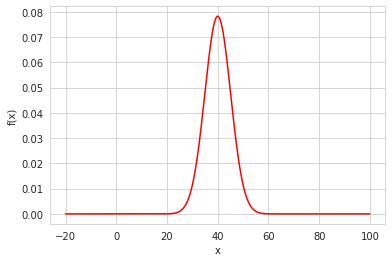
\includegraphics[width=0.9\columnwidth]{Assignment5.png}
    \label{fig:my_label}
\end{figure}


\end{document}
